\documentclass[12pt]{scrartcl}
\usepackage{a4wide}
\usepackage{latexsym}
\usepackage{amssymb}
\usepackage{amsmath}
\usepackage{epic}
\usepackage{graphicx}
\usepackage{enumerate}
\usepackage{float}
\usepackage{amsthm}
\usepackage{diagbox}
\usepackage{hyperref}
\usepackage{mathtools}
\usepackage{biblatex} 

\addbibresource{ref.bib}

\newcommand{\tr}{\mbox{\sf true}}
\newcommand{\fa}{\mbox{\sf false}}
\newcommand{\bimp}{\leftrightarrow}
\newcommand{\NN}{\ensuremath{\mathbb{N}}}
\newcommand{\BB}{\ensuremath{\mathbb{B}}}
\newcommand{\mtt}[1]{\ensuremath{\mathtt{#1}}}
\newcommand{\cnt}{\ensuremath{\mathop{\mathsf{C}}}}
\newcommand{\nt}[1]{\ensuremath{\mtt{next}(#1)}}

\title{Practical assignment: part 2\\Automated Reasoning}
\author{Luko van der Maas\\s1010320\\\href{mailto:l.vandermaas@student.ru.nl}{l.vandermaas@student.ru.nl} }

\setcounter{tocdepth}{3}

\begin{document}
\maketitle

\section{Packet switching network}
\subsection{The problem}
Consider the following packet switching network as introduced in the Appendix of the exercises.
\begin{center}
    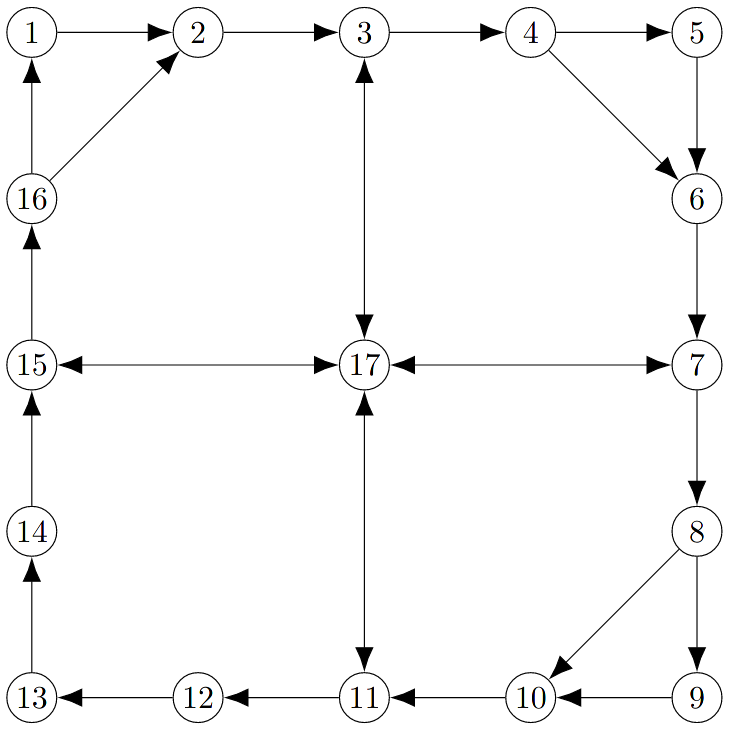
\includegraphics[width=0.5\textwidth]{network.png}
\end{center}
The initial state is defined to be the state in which all channels are free. Investigate whether there is a deadlock reachable from the initial state, for the following choices of the set $M$ of main nodes.
\begin{enumerate}[(a)]
    \item $M=\{1,5,9,13\}$
    \item $M=\{2,4,6\}$
    \item $M=\{1,3,5,15\}$
    \item $M=\{11,13,15\}$
    \item $M=\{11,12,13,15\}$
    \item $M=\{1,8,10\}$
    \item $M=\{5,12,14\}$
    \item $M=\{5,11,14\}$
\end{enumerate}

\subsection{The solution}
\subsubsection{Parameters}
The parameters for this problem are the network $(N,E)$, the routing function $R$ and the main nodes $M$.
We encode the network as pairs of nodes in $N$ for every edge in $E$ in the network. This works as long as every node has at least one edge, but because the network always has a path between every two points this works. The routing function we built as a matrix $R$ of size $|N| \times |N|$ where $R_{ij}$ is the next path to take to get from node $i$ to node $j$. The main nodes we simply encode as a set $M$ of nodes.

\subsubsection{Defining the model}
We will be solving this problem using NuSMV. Thus we will be defining initial states and transition rules.

To make sure that at every step only one node can do one action we introduce two new variables $step$ and $focus$. $step$ will be one of $SEND, RECEIVE, PROCESS$ at all times. $focus$ determines what node can do the action as specified in $step$ and thus always contains a value from $N$. Not all combinations of $step$ and $focus$ are however valid states, only nodes in $M$ can send or receive and only when the edges that are read from are empty or full respectively. Thus we first introduce a third variable and then specify the transition rules for $focus$ and $send$.

To encode the contents of an edge we introduce a new variable $contains$, it is an array of size $|E|$ and has values from $\{\bot\} + N$. Where $\bot$ encodes an empty channel and a value from $N$ encodes a message addressed to the value.

With that information we can encode the transition rules for $focus$ and $step$. We have a rule for when $step = SEND$ and when $step = RECEIVE$:
\begin{align*}
    &\nt{step} = SEND \rightarrow \bigvee_{m\in M}\left( \nt{focus} = m \wedge \bigvee_{d\in (M\setminus m)}\left(contains_{route_{md}} = \bot\right)\right) \\
    &\nt{step} = RECEIVE \rightarrow \bigvee_{m\in M}\left( \nt{focus} = m \wedge \bigvee_{e\in E}\left(e_{\mtt{dest}} = m \rightarrow contains_{e} = m\right)\right)
\end{align*}
There is no initial value specified for $focus$ and $step$ and the only rules that govern there  value are thus the transition rules that are and will be specified.

The initial value for contains for every edge is $\bot$ the transition rules are a bit more involved and broken up in three parts. For every value for $step$ we define the associated transition rules. The rules that are defined are made in such a way that all reachable states are valid states for the network to be in.

We start with the $SEND$ rule. We have to set three things for this rule. That there is an edge on which we want to send something to another main node that is empty, that in the next state that edge is filled with a message addressed to the other main node and that all other edges stay constant. We thus get the following rule:
\begin{align*}
    &\nt{step} \wedge \nt{focus} = m \rightarrow \\
    &\hspace{1cm}\bigvee_{d\in (M\setminus m)}\left(
        \begin{array}{l}
            contains_{route_{md}} = 0 \wedge \nt{contains_{route_{md}}} = d\ \wedge \\
            \bigwedge_{e\in (E\setminus route_{md})}\left( \nt{contains_e} = contains_e\right)
        \end{array}
    \right)
\end{align*}

The $RECEIVE$ step is very similar except that we make sure that for main node $m$, there is a edge that has a package addressed to $m$ in it, that in the next state that edge is empty and all other edges stay constant:
\begin{align*}
    &\nt{step} \wedge \nt{focus} = m \rightarrow \\
    &\hspace{1cm}\bigvee_{e\in (E)}\left( e_{\mtt{dest}} = m \rightarrow
        \begin{array}{l}
            contains_{e} = m \wedge \nt{contains_{e}} = \bot\ \wedge \\
            \bigwedge_{o\in (E\setminus route_{md})}\left( \nt{contains_o} = contains_o\right)
        \end{array}
    \right)
\end{align*}

The $PROCCESS$ step is a bit more complicated as it has to modify two edges to there appropriated values. For the current node that has focus $n$ we make sure there is an edge with destination $n$ that contains an $m\in M$ and that the next value of that edge is $\bot$. Then we also ensure that the current value of the edge that the packet is routed to is empty and then in the next state fill it with the packet:
\begin{align*}
    &\nt{step} \wedge \nt{focus} = n \rightarrow \\
    &\hspace{1cm}\bigvee_{e\in (E)}\left( e_{\mtt{dest}} = n \rightarrow
        \begin{array}{l}
            contains_{e} = m \wedge \nt{contains_{e}} = \bot\ \wedge \\
            contains_{route_{nm}} = \bot \wedge \nt{contains_{route_{nm}}} = m\ \wedge \\
            \bigwedge_{o\in (E\setminus route_{md} \setminus e)}\left( \nt{contains_o} = contains_o\right)
        \end{array}
    \right)
\end{align*}

\subsubsection{Combining all clauses}
Now that we have defined all needed clauses we can put them all together in a model. We have to do an and over either all main nodes or all nodes.
\begin{align*}
    &\nt{step} = SEND \rightarrow \bigvee_{m\in M}\left( \nt{focus} = m \wedge \bigvee_{d\in (M\setminus m)}\left(contains_{route_{md}} = \bot\right)\right) & \wedge \\
    &\nt{step} = RECEIVE \rightarrow \bigvee_{m\in M}\left( \nt{focus} = m \wedge \bigvee_{e\in E}\left(e_{\mtt{dest}} = m \rightarrow contains_{e} = m\right)\right)  & \wedge \\
    &\bigwedge_{m\in M} \left(
        \begin{array}{l}
            \nt{step} \wedge \nt{focus} = m \rightarrow \\
            \hspace{1cm}\bigvee_{d\in (M\setminus m)}\left(
                \begin{array}{l}
                    contains_{route_{md}} = 0 \wedge \nt{contains_{route_{md}}} = d\ \wedge \\
                    \bigwedge_{e\in (E\setminus route_{md})}\left( \nt{contains_e} = contains_e\right)
                \end{array}
                \right)
        \end{array}
    \right) &\wedge \\
    &\bigwedge_{m\in M} \left(
        \begin{array}{l}
            \nt{step} \wedge \nt{focus} = m \rightarrow \\
            \hspace{1cm}\bigvee_{e\in (E)}\left( e_{\mtt{dest}} = m \rightarrow
                \begin{array}{l}
                    contains_{e} = m \wedge \nt{contains_{e}} = \bot\ \wedge \\
                    \bigwedge_{o\in (E\setminus route_{md})}\left( \nt{contains_o} = contains_o\right)
                \end{array}
            \right)
        \end{array}
    \right) &\wedge \\
    &\bigwedge_{n\in N} \left(
        \begin{array}{l}
            \nt{step} \wedge \nt{focus} = n \rightarrow \\
            \hspace{1cm}\bigvee_{e\in (E)}\left( e_{\mtt{dest}} = n \rightarrow
                \begin{array}{l}
                    contains_{e} = m \wedge \nt{contains_{e}} = \bot\ \wedge \\
                    contains_{route_{nm}} = \bot \wedge \nt{contains_{route_{nm}}} = m\ \wedge \\
                    \bigwedge_{o\in (E\setminus route_{md} \setminus e)}\left( \nt{contains_o} = contains_o\right)
                \end{array}
            \right)
        \end{array}
    \right)
\end{align*} 

\subsubsection{Converting to NuSMV}
We can use a templating engine (I used jinja) to covert our model to nusmv syntax. The only tricky part is the $\bot$ value for contains. We use the number 0 to model this. However as we use this number as a index in other arrays we have to make sure that all arrays have an index 0. In the route function we set the route of 0 to 0 everywhere.

\subsubsection{Solving the problem}
To now solve the problem we check if the model is deadlock free with the check\_fsm command. If there are no deadlocks in the reachable states there is no deadlock in the model and no deadlock in the network with the specified main nodes. 

For some reason when we have more then 3 main nodes in the model NuSMV does not manage to build the model. After waiting multiple hours the cpu usage drops down to almost nothing but there is no result. I have no idea why that happens as with three main nodes it builds the model in around ten seconds. This resulted in a few of the questions having no answer. I would be very interested in hearing why it dit not work for more then 3 nodes.

\paragraph{results}
\begin{enumerate}[(a)]
    \item no result
    \item deadlock
    \item no result
    \item deadlock free
    \item no result
    \item deadlock
    \item deadlock
    \item deadlock free
\end{enumerate}

\subsubsection{Computation time}
The total computation time with three nodes is around 5 minutes. With four main nodes NuSMV itself seems to deadlock and thus the computation does not finish.

\section{Villages}
\subsection{The problem}
Three non-self-supporting villages A, B and C in the middle of nowhere consume one food package each per time unit.  The required food packages are delivered by a truck,having  a  capacity  of  300  food  packages.   The  locations  of  the  villages  are  given  in the following picture, in which the numbers indicate the distance, more precisely, the number of time units the truck needs to travel from one village to another, including loading or delivering.  The truck has to pick up its food packages at location S containing an unbounded supply.  The villages only have a limited capacity to store food packages:for A and B this capacity is 120, for C it is 200.  Initially, the truck is in S and is fully loaded, and in A, B and C there are 40, 30 and 145 food packages, respectively.
\begin{enumerate}[(a)]
    \item Show that it is impossible to deliver food packages in such a way that each of the villages consumes one food package per time unit forever.
    \item Show  that  this  is  possible  if  the  capacity  of  the  truck  is  increased  to  320  food packages.
    \item Figure out whether it is possible if the capacity of the truck is set to 318.
\end{enumerate}

\subsection{The solution}
The solution to this problem was preceded by to other attempts in NuSMV. Only after making them I found out that this does not work. I then transplanted the base formulas to z3 and added the loop searching. This is the result.

\subsubsection{Parameters}
To generalize this problem we parametrize the graph of villages and the supply depot, $(V,E)$. We do this by simply making an array of distances between all nodes $v\in V$ in the graph. We also store the initial and max capacity for all villages and the max capacity for the truck.
\begin{align*}
    &distances = \left(
        \begin{array}{llll}
            \bot & 29& 21& \bot \\
            29& \bot & 17& 32 \\
            21& 17& \bot & 37 \\
            \bot & 32& 37& \bot 
        \end{array}
    \right) \\
    &v\_cap = \left(
        \begin{array}{llll}
            \bot& 120& 120& 200
        \end{array}
    \right) \\
    &v\_init\_cap = \left(
        \begin{array}{llll}
            \bot& 40& 30& 145
        \end{array}
    \right)\\
    &t\_max\_cap = 30
\end{align*}
The first value in distances, capacity, and initial capacity are always the supply depot and thus have no capacity and initial capacity.

\subsubsection{Defining the model}
Because we are searching for loops, all variables in the model have a time dimension and we define a time bound. The time bound is the maximum amount of steps we look at for a loop in which all villages always have food. 

We have three variables in our model the truck contents $truck$, the villages contents $vil$ and the location of the truck $loc$. All variables can have a an extra $_t$ to denote the value of this variable at time $t$.

We start by defining the constraints on $loc$. The truck starts at the supply depot thus at time 0 $loc$ should be 0:
\begin{align*}
    loc_0 = 0
\end{align*}
For any other time we should only be able to change $loc$ in time $t+1$ if the distance from $loc_t$ to $loc_{t+1}$ is not $\bot$.
\begin{align*}
    \bigvee_{v\in V}\left(distances_{loc_t, v} \geq 0 \wedge loc_{t+1} = v \right)
\end{align*}

Next we look at the truck contents. There are two cases for the truck content, if we are at the supply depot we set the truck contents to the max capacity, if we are not at a supply depot, the truck contents has to be lower or equal then the previous truck contents. It should also always be between 0 and $t\_max\_cap$\footnote{The max bound is not necessary because of the other restrictions but because of clarity we let it stay.}:
\begin{align*}
    &\bigwedge_{t = 0}^{time\_bound + 1} \left(
        0 \leq truck_t \leq t\_max\_cap
    \right) \\
    &truck_0 = t\_max\_cap\\
    &\bigwedge_{t = 0}^{time\_bound} \left(
        truck_{t+1} = \begin{cases}
            truck_{t+1} = t\_max\_cap & \text{if } loc_{t+1} = 0 \\
            truck_{t+1} \leq truck_t & \text{else}
        \end{cases}
    \right)
\end{align*}

Lastly we have the most difficult set of rules, the rules for the contents of the villages $vil$. We can set the initial values for the villages according to $v\_init\_cap$. Also at every time $t$ $vil_v$ for a villages $v$ should be between 0 and $v\_max\_cap$. Those are the easy ones, now for the more difficult transition relation between a time $t$ and $t+1$. We set the new value for a villages $v$ by subtracting the distance between the current and next location from the contents of $v$. We then look at if the truck will arrive at $v$ in the next step and that the current capacity minus the distance is more then 0 and if so add the difference between the current and next truck contents, otherwise add 0. This ensures that we don't run out of food during the trip but then with the new food we get above 0 again.
\begin{align*}
    &vil_{0,v} = v\_init\_cap_v\\
    &\bigwedge_{t = 0}^{time\_bound + 1} \left(0 \leq vil_{t,v} \leq v\_cap_v\right)\\
    &\bigwedge_{t = 0}^{time\_bound} \left(\begin{array}{ll}
        vil_{t+1,v} = &vil_{t,v} - distances_{loc_t, loc_{t+1}} + \\
        &\begin{cases}
            truck_t - truck_{t+1} & \text{if } \begin{array}{l}
                loc_{t+1} = v \wedge\\
                vil_{t,v} - distances_{loc_t, loc_{t+1}} \geq 0
            \end{array}\\
            0 &\text{else}
        \end{cases}
    \end{array}
    \right)
\end{align*}

Now that we have defined our rules surrounding the villages and trucks we just have to find a loop. We have defined the model in such a way that a invalid state always results in no more available steps, thus we can just look for two different times $t_1$ and $t_2$ where $vil$, $truck$ and $loc$ are all equal.
\begin{align*}
    vil_{t_1} &= vil_{t_2} \wedge \\
    truck_{t_1} &= truck_{t_2} \wedge \\
    vil_{t_1} &= vil_{t_2}
\end{align*}

\subsubsection{Combining all clauses}
Now that we have all the clauses we can apply them over all villages where needed.
\begin{align*}
    & loc_0 = 0 & \wedge \\
    & \bigwedge_{t= 0}^{time\_bound} \bigvee_{v\in V}\left(distances_{loc_t, v} \geq 0 \wedge loc_{t+1} = v \right) & \wedge \\
    &\bigwedge_{t = 0}^{time\_bound + 1} \left(
        0 \leq truck_t \leq t\_max\_cap
    \right) & \wedge \\
    &truck_0 = t\_max\_cap & \wedge \\
    &\bigwedge_{t = 0}^{time\_bound} \left(
        truck_{t+1} = \begin{cases}
            truck_{t+1} = t\_max\_cap & \text{if } loc_{t+1} = 0 \\
            truck_{t+1} \leq truck_t & \text{else}
        \end{cases}
    \right) & \wedge \\
    &\bigwedge_{v\in V}\left( vil_{0,v} = v\_init\_cap_v\right) & \wedge\\
    &\bigwedge_{v\in V}\bigwedge_{t = 0}^{time\_bound + 1} \left(0 \leq vil_{t,v} \leq v\_cap_v\right)& \wedge\\
    &\bigwedge_{v\in V}\bigwedge_{t = 0}^{time\_bound} \left(\begin{array}{ll}
        vil_{t+1,v} = &vil_{t,v} - distances_{loc_t, loc_{t+1}} + \\
        &\begin{cases}
            truck_t - truck_{t+1} & \text{if } \begin{array}{l}
                loc_{t+1} = v \wedge\\
                vil_{t,v} - distances_{loc_t, loc_{t+1}} \geq 0
            \end{array}\\
            0 &\text{else}
        \end{cases}
    \end{array}
    \right) & \wedge \\
    &\bigvee_{t_1 = 0}^{time\_bound} \bigvee_{t_2 = 1}^{t_1}\left(
        \begin{array}{ll}
            vil_{t_1} = vil_{t_2} & \wedge \\
            truck_{t_1} = truck_{t_2} & \wedge \\
            vil_{t_1} = vil_{t_2}
        \end{array}
    \right)
\end{align*}

\subsubsection{Converting to z3} 
As usual we can transform our model fairly one to one to z3, there are just a few things we should watch out for. First to create our time dependant variables we create a vector of variables one for each time step plus one for the final step. We also add a variable for distances were we would normally hardcode it during generation and set it to be exactly equal to the distances matrix. We have to do this because the index to this array is a variable and not a constant. All other parameters can be hardcoded.

There is one more thing we do to be able to easily interpret the results, we add two variables $loop\_start$ and $loop\_end$ that are equal to $t_1$ and $t_2$ when there is a loop. We can then use these variables when result has been given to see where the loop is.

\subsubsection{Results}
We check with a time bound of 20 as this is more then enough for both (b) and (c). With this time bound we find no loop where all villages stay alive for (a). For (b) we find a loop:
\begin{verbatim}
    --------- Time 0 ---------
    truck location = S
    truck content = 320
    village A = 40 
    village B = 30 
    village C = 145 
    --------- Time 1 ---------
    truck location = B
    truck content = 212
    village A = 19 
    village B = 117 
    village C = 124 
    --------- Time 2 ---------
    truck location = A
    truck content = 95
    village A = 119 
    village B = 100 
    village C = 107 
    --------- Time 3 ---------
    truck location = B
    truck content = 58
    village A = 102 
    village B = 120 
    village C = 90 
    --------- Time 4 --------- <- Loop starts here
    truck location = S
    truck content = 320
    village A = 81 
    village B = 99 
    village C = 69 
    --------- Time 5 ---------
    truck location = A
    truck content = 252
    village A = 120 
    village B = 70 
    village C = 40 
    --------- Time 6 ---------
    truck location = C
    truck content = 66
    village A = 88 
    village B = 38 
    village C = 194 
    --------- Time 7 ---------
    truck location = B
    truck content = 0
    village A = 51 
    village B = 67 
    village C = 157 
    --------- Time 8 ---------
    truck location = S
    truck content = 320
    village A = 30 
    village B = 46 
    village C = 136 
    --------- Time 9 ---------
    truck location = A
    truck content = 202
    village A = 119 
    village B = 17 
    village C = 107 
    --------- Time 10 ---------
    truck location = B
    truck content = 82
    village A = 102 
    village B = 120 
    village C = 90 
    --------- Time 11 --------- <- Loop ends here
    truck location = S
    truck content = 320
    village A = 81 
    village B = 99 
    village C = 69
\end{verbatim}
For (c) we find a similar loop which also a size of 11:
\begin{verbatim}
    --------- Time 0 ---------
    truck location = S
    truck content = 318
    village A = 40 
    village B = 30 
    village C = 145 
    --------- Time 1 ---------
    truck location = B
    truck content = 210
    village A = 19 
    village B = 117 
    village C = 124 
    --------- Time 2 ---------
    truck location = A
    truck content = 92
    village A = 120 
    village B = 100 
    village C = 107 
    --------- Time 3 ---------
    truck location = B
    truck content = 55
    village A = 103 
    village B = 120 
    village C = 90 
    --------- Time 4 --------- <- Loop starts here
    truck location = S
    truck content = 318
    village A = 82 
    village B = 99 
    village C = 69 
    --------- Time 5 ---------
    truck location = A
    truck content = 252
    village A = 119 
    village B = 70 
    village C = 40 
    --------- Time 6 ---------
    truck location = C
    truck content = 66
    village A = 87 
    village B = 38 
    village C = 194 
    --------- Time 7 ---------
    truck location = B
    truck content = 0
    village A = 50 
    village B = 67 
    village C = 157 
    --------- Time 8 ---------
    truck location = S
    truck content = 318
    village A = 29 
    village B = 46 
    village C = 136 
    --------- Time 9 ---------
    truck location = A
    truck content = 198
    village A = 120 
    village B = 17 
    village C = 107 
    --------- Time 10 ---------
    truck location = B
    truck content = 78
    village A = 103 
    village B = 120 
    village C = 90 
    --------- Time 11 --------- <- Loop ends here
    truck location = S
    truck content = 318
    village A = 82 
    village B = 99 
    village C = 69 
\end{verbatim}

\subsubsection{Computation time}
The computation time is around 5 seconds for both (b) and (c). For (a) it takes about 30 seconds to find no loop to time bound 20.

\section{Rewriting}
\subsection{Problem a}
We can encode the rewrite rules of the problem in a similar manner as done in the lecture. We have a predicate $R(x,y)$ that defines the rule $x \rightarrow y$ and the predicate $RR(x,y)$ that says $x \rightarrow^\star y$. With those strategies we get the following encoding:
\begin{verbatim}
    formulas(assumptions).
    R(a(x, x), x).
    R(a(x, y), a(y, x)).
    R(a(x,  a(y, z)), a(a(x, y), z)).
    R(x, y) -> R(a(x, z), a(y, z)).
    R(x, y) -> R(a(z, x), a(z, y)).
    RR(x, x).
    (RR(x, y) & R(y, z)) -> RR(x, z).
    end_of_list.
    formulas(goals).
    R(a(p, a(q, a(p, a(q, a(p,  a(q, p)))))), a(p, q)).
    end_of_list.
\end{verbatim}

When we put this through mace4 we get a counterexample and thus the goal does not hold and we can't rewrite $a(p, a(q, a(p, a(q, a(p,  a(q, p))))))$ to $a(p, q)$. The model for the counterexample is of size 3.

This was calculated in very little time as it was a trivial counterexample.

\subsection{Problem b}
For problem b we input the formula's as written in the assumptions of our input for prover9 and mace4. We also define I as an operator to make sure that it is not a variable but an element. We then also add commutativity as goal.
\begin{verbatim}
    op(325, infix, ~).
    op(340, ordinary, I).

    formulas(assumptions).
    x ~ (y ~ z) = (x ~ y) ~ z.
    x ~ I = x.
    I ~ x = x.
    end_of_list.
    formulas(goals).
    x ~ y = y ~ x.
    end_of_list.
\end{verbatim}
Now for each of the subquestions we add the appropriate extra assumption.
\begin{verbatim}
a:  op(325, infix, ~).
    op(340, ordinary, I).

    formulas(assumptions).
    x ~ (y ~ z) = (x ~ y) ~ z.
    x ~ I = x.
    I ~ x = x.
    x ~ x = I.
    end_of_list.
    formulas(goals).
    x ~ y = y ~ x.
    end_of_list.

b:  op(325, infix, ~).
    op(340, ordinary, I).

    formulas(assumptions).
    x ~ (y ~ z) = (x ~ y) ~ z.
    x ~ I = x.
    I ~ x = x.
    x ~ (x ~ x) = I.
    end_of_list.
    formulas(goals).
    x ~ y = y ~ x.
    end_of_list.

c:  op(325, infix, ~).
    op(340, ordinary, I).

    formulas(assumptions).
    x ~ (y ~ z) = (x ~ y) ~ z.
    x ~ I = x.
    I ~ x = x.
    (x ~ x) ~ (x ~ x) = I.
    end_of_list.
    formulas(goals).
    x ~ y = y ~ x.
    end_of_list.
\end{verbatim}
When we run it through prover9 and mace4 we get the following results:
\begin{enumerate}[(a)]
    \item proven
    \item disproven (size 27)
    \item disproven (size 8)
\end{enumerate}
All results were calculated in at most a few seconds, the smell counterexample example in under one second.

\section{The game Set}
\subsection{The problem}
There exists the well known game Set. It consists of 81 cards with a picture on each. These pictures differ in four categories: shape, colour, fill and amount of shapes. Each property has 3 possible options such that we get $3^4 = 81$ different possible cards. The possible options for each property are:
\begin{description}
    \item[count] 1, 2, 3
    \item[shape] oval, diamond, squiggle
    \item[fill] empty, shaded, filled
    \item[colour] purple, red, green 
\end{description}

The game now consists of finding three cards where for every property either they are all different or they are all equal. We start with 9 cards and if no sets are found we lay down one more card till someone finds a set. The person with the most sets when we are through the cards is the winner. An example board can be found in figure \ref*{fig:set}

\begin{figure}[h]
    \centering
    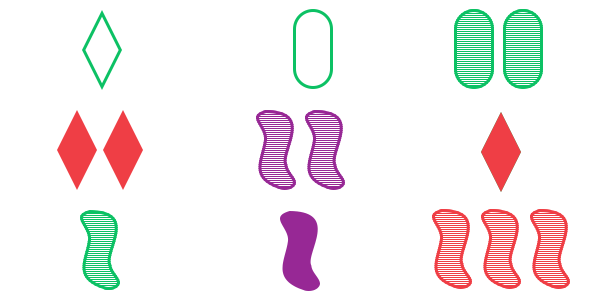
\includegraphics[width=0.5\textwidth]{set_board.png}
    \caption{A set board of 9 cards with at least one set: green 1 shaded squiggle, purple 2 shaded squiggle, red 3 shaded squiggle}
    \label{fig:set}
\end{figure}

\paragraph{problem a}
The first problem we would now like to solve is if there exists a board of a set amount of cards in which there is no set, and we would like to see it if it exists.

\paragraph{}
This is a fairly simple game and new more difficult variations have been made, these variations all define new types of sets that can be found\footnote{These variations are not thought of by me, but come from Stichting Vierkant voor Wiskunde}. The first variation is: find two non identical pairs of cards that both miss the same card to complete a set. We will call this a second order set and the firs type of set thus a first order set. There actually exists a second order set in figure \ref*{fig:set}. The first pair is purple squiggle filled 1 and shaded 2, the second pair is diamond filled 1 red and oval shaded 2 green, both these pairs miss squiggle empty 3 purple. 

\paragraph{problem b}
We again want to know for a certain amount of cards if there always exists a second order set.

\paragraph{}
There also exists a third type of set, which we will call the third order set. This set consists of three non identical pairs where the cards they are missing to create a set again form a set. A first order set is actually also a third order set if you take all combinations of the cards as the three pairs.

\paragraph{problem c}
We want to know if for a certain amount of cards there exists a third order set.

\subsection{The solution}
\subsubsection{Parameters}
To solve these problems more generally we let there be any number of properties with 3 variations for each. Letting there be more or less then 3 variations for any property creates a lot more difficult constraints as we can't easily find the missing card for a set. Our two parameters are thus $T$: 
\begin{description}
    \item[count] 1, 2, 3
    \item[shape] oval, diamond, squiggle
    \item[fill] empty, shaded, filled
    \item[colour] purple, red, green 
\end{description}
and $card\_count$.

\subsubsection{Encoding the variables}
To encode the properties of a card we create a new datatype that is the combination of the value for all four properties:
\begin{align*}
    Card := \bigtimes_{t\in T} T_t
\end{align*}
We can now create a vector of cards $C$ of size $card\_count$ to encode our Set cards.

\subsubsection{Defining the model}
There is one common constraint in Set for all types of Sets, all cards in the game are unique. Thus our first constraint is:
\begin{align*}
    \mtt{Distinct}(C)
\end{align*}

We can now start defining for each type of set when it occurs, we then take the inverse of the constraint to get our clause. 

It also took some time to find the proper way to define the 2 new types of sets, and those were influenced by different attempts at making the clauses. Thus the wording in the problem description matches the clauses exactly as that was what we found the most clear way to define them and also write them down in predicate logic with \mtt{Distinct}

\paragraph{First order sets}
are pretty trivial as we just for every property say that they should all be distinct or equal. Thus for every combination of 3 cards $a, b, c$ this should hold
\begin{align*}
    \neg \bigwedge_{t\in T} \left( a_t = b_t = c_t \vee \mtt{Distinct}(a_t, b_t, c_t)\right)
\end{align*}

\paragraph{Second order sets}
are a bit more difficult and we will use a way to find what the third card in a set should be. We first tried to do this using an exists, this would have also allowed us to drop the 3 options per property constraint. However the solving strategies for exists in z3 are not complete and thus sometimes z3 would find unsat when there did exist a board with no sets.

What we do now is look at the remaining value for every property of the two pairs and make sure they are not equal. We need some more notation to get the $n$ value of a specific type $t$: $t_n$, then we introduce a $last\_card$ function that is defined as:
\begin{align*}
    last\_card(t,a,b) = \begin{cases}
        a_t & \text{if } a_t = b_t \\
        t_0 & \text{if } \mtt{Distinct}(t_0, a_t, b_t) \\
        t_1 & \text{if } \mtt{Distinct}(t_1, a_t, b_t) \\
        t_2 & \text{if } \mtt{Distinct}(t_2, a_t, b_t)
    \end{cases}
\end{align*}
As there are only three options these are mutually exclusive and thus well defined. We can now create our clause for second order sets on two non identical pairs, $(a,b), (c,d)$
\begin{align*}
    \neg \bigwedge_{t\in T} \left(last\_card(t, a,b) = last\_card(t, c,d) \right)
\end{align*}

\paragraph{third order sets}
For third order sets we use much the same strategy as the second order sets, just with the constraints of the first order sets on the results of $last\_card$ on our three non identical pairs $(a,b), (c,d), (e,f)$:
\begin{align*}
    \neg \bigwedge_{t\in T} \left(\begin{array}{ll}
        last\_card(t,a,b) = last\_card(t,c,d) = last\_card(t,e,f) &\vee\\
        \mtt{Distinct}(last\_card(t,a,b), last\_card(t,c,d), last\_card(t,e,f))
    \end{array}
    \right)
\end{align*}

\paragraph{Optimisations}
These four clauses work well to find a board with no sets if that exists, however if it does not exist it will take a very long time to prove this. This is the case because there are many symmetries in Set. When looking at the statistics of z3 we find that it seems like it tries almost all different options when it tries to prove unsat. Thus we want to remove symmetries without reducing completeness of the algorithm. This is however quite a hard problem as for twenty cards there are still 682344 configurations without first order sets, but there are no configurations of 21 cards without first order sets\cite{Davis2003TheCG}.

We managed to restrict the first two cards to all needed possible states. We do this by thinking of the cards as if we are laying them down one by one. The first card does not matter, because no matter what we choose all other options are still open. Thus we can set the first card to a specific card. The second card we can't set to one specific card as we would then be removing non symmetric options for sets. However the only thing that is important for all properties is if it is the same or different then the other cards, and since we are laying them down one at a time we only have to thing about the first card. For every property we thus let it either be the same or different, when it is the same only one option exists. When they are different two options exists which are again symmetric, thus we just choose the first one. There is however one more symmetry in these two cards, the properties are identical, thus having the properties be: (same, same, different, same) is symmetric to (same, same, same, different). The only thing that matters is the amount of same and different properties. Thus we say that we only want the properties to first be different then same. That way we only have one order.
\begin{align*}
    &\bigwedge_{t\in T} C^0_t = t_0\\
    &\bigwedge_{i=0}^{|T|}\left( C^1_{T^i} = C^0_{T^i} \rightarrow \bigwedge_{t\in T^{\langle i,\rightarrow\rangle}} C^1_t = C^0_t \right)
\end{align*}
Here we use a superscript to denote an index in a list and and a range to denote a subset of a list those indices. 

I suspect that this also works for all indices where we reference the previous card, thus:
\begin{align*}
    &\bigwedge_{j=1}^{|C|}\bigwedge_{i=0}^{|T|}\left( C^j_{T^i} = C^{j-1}_{T^i} \rightarrow \bigwedge_{t\in T^{\langle i,\rightarrow\rangle}} C^j_t = C^{j-1}_t \right)
\end{align*}
However, I have not been able to thing of a proof why this would work, it is just an intuition and thus is not used.

\subsubsection{Combining the model}
In our descriptions of the clauses we used the wording combinations of cards quite a few times, this is however not easily represented using set operations. We thus introduce a new function $\mtt{comb}(S, n)$ that gives all size $n$ combinations in $S$. We can do this as it is not part of the logical formula as put into z3 and handled by our scripting language.
\begin{align*}
    &\mtt{Distinct}(C) \wedge \\
    &\bigwedge_{(a,b,c)\in\mtt{comb}(C,3)}\left(
        \neg \bigwedge_{t\in T} \left( a_t = b_t = c_t \vee \mtt{Distinct}(a_t, b_t, c_t)\right)
    \right) \wedge \\
    &\bigwedge_{(a,b)\in\mtt{comb}(C,2)}\bigwedge_{(c,d)\in\mtt{comb}(C,2)\setminus(a,b)} \left(
        \neg \bigwedge_{t\in T} \left(
            \begin{cases}
                a_t & \text{if } a_t = b_t \\
                t_0 & \text{if } \mtt{Distinct}(t_0, a_t, b_t) \\
                t_1 & \text{if } \mtt{Distinct}(t_1, a_t, b_t) \\
                t_2 & \text{if } \mtt{Distinct}(t_2, a_t, b_t)
            \end{cases} = \begin{cases}
                c_t & \text{if } c_t = d_t \\
                t_0 & \text{if } \mtt{Distinct}(t_0, c_t, d_t) \\
                t_1 & \text{if } \mtt{Distinct}(t_1, c_t, d_t) \\
                t_2 & \text{if } \mtt{Distinct}(t_2, c_t, d_t)
            \end{cases}
        \right)
    \right) \wedge \\
    &\bigwedge_{(a,b)\in\mtt{comb}(C,2)}\bigwedge_{(c,d)\in\mtt{comb}(C,2)\setminus(a,b)}\bigwedge_{(e,f)\in\mtt{comb}(C,2)\setminus(a,b)\setminus(c,d)}\\ &\hspace{1cm} \left(
        \neg \bigwedge_{t\in T} \left(\begin{array}{ll}
            \begin{cases}
                a_t & \text{if } a_t = b_t \\
                t_0 & \text{if } \mtt{Distinct}(t_0, a_t, b_t) \\
                t_1 & \text{if } \mtt{Distinct}(t_1, a_t, b_t) \\
                t_2 & \text{if } \mtt{Distinct}(t_2, a_t, b_t)
            \end{cases} = \begin{cases}
                c_t & \text{if } c_t = d_t \\
                t_0 & \text{if } \mtt{Distinct}(t_0, c_t, d_t) \\
                t_1 & \text{if } \mtt{Distinct}(t_1, c_t, d_t) \\
                t_2 & \text{if } \mtt{Distinct}(t_2, c_t, d_t)
            \end{cases} =&\\ \hspace{1cm}\begin{cases}
                e_t & \text{if } e_t = f_t \\
                t_0 & \text{if } \mtt{Distinct}(t_0, e_t, f_t) \\
                t_1 & \text{if } \mtt{Distinct}(t_1, e_t, f_t) \\
                t_2 & \text{if } \mtt{Distinct}(t_2, e_t, f_t)
            \end{cases} &\vee\\
            \mtt{Distinct}(\begin{cases}
                a_t & \text{if } a_t = b_t \\
                t_0 & \text{if } \mtt{Distinct}(t_0, a_t, b_t) \\
                t_1 & \text{if } \mtt{Distinct}(t_1, a_t, b_t) \\
                t_2 & \text{if } \mtt{Distinct}(t_2, a_t, b_t)
            \end{cases}, \begin{cases}
                c_t & \text{if } c_t = d_t \\
                t_0 & \text{if } \mtt{Distinct}(t_0, c_t, d_t) \\
                t_1 & \text{if } \mtt{Distinct}(t_1, c_t, d_t) \\
                t_2 & \text{if } \mtt{Distinct}(t_2, c_t, d_t)
            \end{cases},&\\\hspace{1cm} \begin{cases}
                e_t & \text{if } e_t = f_t \\
                t_0 & \text{if } \mtt{Distinct}(t_0, e_t, f_t) \\
                t_1 & \text{if } \mtt{Distinct}(t_1, e_t, f_t) \\
                t_2 & \text{if } \mtt{Distinct}(t_2, e_t, f_t)
            \end{cases})
        \end{array}
        \right)
    \right) \wedge \\
    &\bigwedge_{t\in T} C^0_t = t_0 \wedge\\
    &\bigwedge_{i=0}^{|T|}\left( C^1_{T^i} = C^0_{T^i} \rightarrow \bigwedge_{t\in T^{\langle i,\rightarrow\rangle}} C^1_t = C^0_t \right)
\end{align*}

\subsubsection{Convert to z3}
We use the z3 datatypes to model a card. The combinations we make using the python itertools library and the set minus is done simply by using if statements. All other functions are directly translated to z3.

To check the different problems we include the different order set clauses if we want to test for them.

\subsubsection{Results}
We can find a solution for first order sets with 20 cards as seen in figure \ref*{fig:1-20}. For 21 cards even with our optimisations we still are not able to get unsat from z3. However we do know that it is unsat as otherwise there would have been a sat result in under an hour.

\begin{figure}[h]
    \centering
    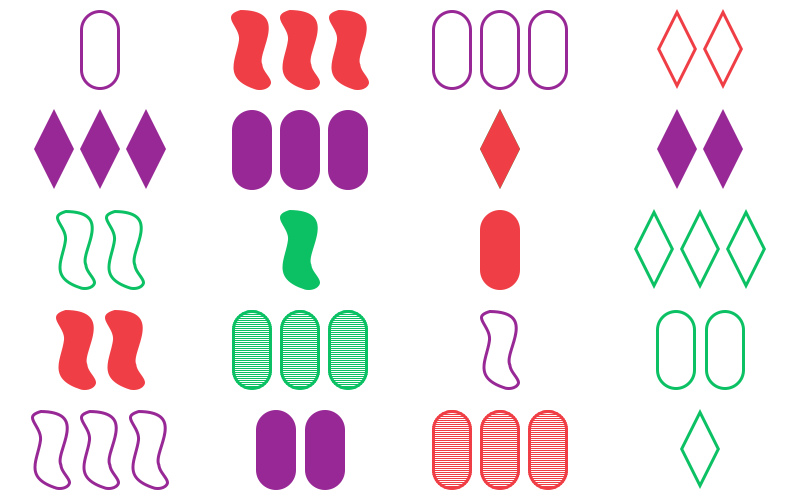
\includegraphics[width=0.5\textwidth]{../set/board_20_1_nd}
    \caption{20 set cards with no first order set in it.}
    \label{fig:1-20}
\end{figure}

For second order sets we are able to get sat results for up to 9 cards with a 9 card board being shown in figure \ref*{fig:2-9}. Again no unsat is actually found as we have not applied enough optimisations yet but there it is clear no will be found either.

\begin{figure}[h]
    \centering
    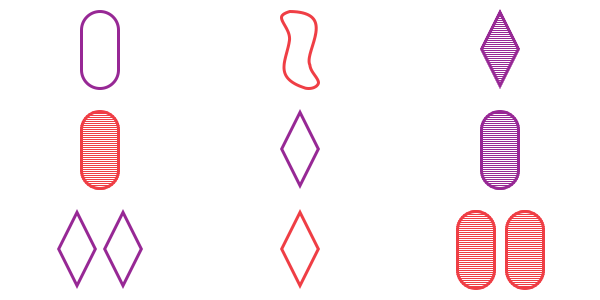
\includegraphics[width=0.5\textwidth]{../set/board_9_1_nd}
    \caption{9 set cards without a second order set.}
    \label{fig:2-9}
\end{figure}

For third order sets when we lay down 7 cards there are actually already always third order sets in there. When we check for all three types of sets at the same time we get the same result. That is obvious for the first order sets as they are also third order sets. However, it is interesting for the second order sets as they are not trivially also third order sets. An example of a 6 card board with no third order sets and one with no first, second or third order sets can be found in figure \ref*{fig:3-6} and \ref*{fig:123-6} respectively.
 
\begin{figure}[h]
    \centering
    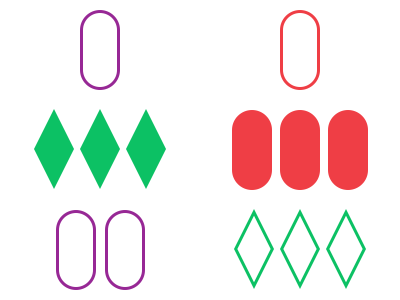
\includegraphics[width=0.5\textwidth]{../set/board_6_3_d}
    \caption{6 set cards with no third order set.}
    \label{fig:3-6}
\end{figure}

\begin{figure}[h]
    \centering
    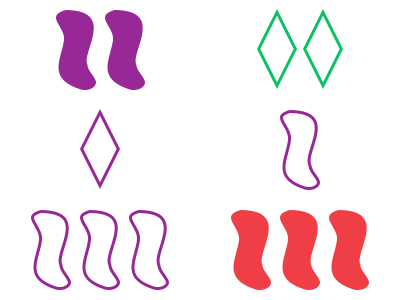
\includegraphics[width=0.5\textwidth]{../set/board_6_123_d}
    \caption{6 set cards with no first, second or third order set.}
    \label{fig:123-6}
\end{figure}

\subsubsection{Computation time}

The computation time for first order sets is very respectable and even with 20 cards it is done in 102 second of which 2 was building the model. For 3 cards it takes a total of 0.032 seconds. With 21 cards we have let it run for more then a day with no results but the statistics tells us it is probably doing a lot of backtracking. For the second order sets we have basically the same story. As we have quite a few less cards it takes a bit less time. However, it is a lot more clauses as we can make a lot more combinations. This is especially the case for the third order sets as they have many options just making the constraints actually takes the most time with 64 seconds of the total 70 seconds needed for the 6 card case.

\section{Sources}

\printbibliography

\end{document}
